\chapter{Экспериментальный раздел}
\label{cha:research}

В рамках дипломного проекта был проведен ряд экспериментов, направленных на исследование описанных алгоритмов классификации с целью определения наиболее подходящего для решения поставленной задачи.

В ходе работы были рассмотрены следующие алгоритмы классификации: алгоритм опорных векторов, алгоритм $k$-ближайших соседей, алгоритм "наивной"\space Байесовской классификации. Для сравнения эффективности работы алгоритмов были использованы метрики, описанные в аналитическом разделе. 

Так как для решения поставленной задачи используются алгоритмы классификации, реализованные в библиотеке Scikit-Learn, то для сравнения описанных алгоритмов между собой необходимо сначала сравнить эффективность работы алгоритмов в отдельности при различных конфигурациях параметров, предоставляемых используемой библиотекой.

\section{Алгоритм опорных векторов}
Согласно документации Scikit-Learn, конструктор класса SVС, описывающий модель классификатора с использованием алгоритма опорных векторов, принимает два основных параметра, характеризующих модель: $C$ и $kernel$. Параметр $C$ минимизирует величину ошибки обучения, т.е. повышение данного параметра приводит к построению более сложной, но в то же время, более корректной гиперплоскости, однако при слишком высоких значениях данного параметра возможно переобучение сети. 
Параметр $kernel$ определят тип функции ядра, которая используется в случае линейной неразделимости точек в пространстве признаков. Может принимать следующие значения: 'linear', 'rbf', 'poly', 'sigmoid'. 

Библиотека Scikit-Learn предоставляет метод GridSearchCV, позволяющий провести обучение при различных конфигурация параметров модели и оценить эффективность работы с использованием метода перекрестной проверки. Метод перекрестной проверки основан на разделении обучающей выборки на $k$ подвыборок, каждая из которых $k-1$ раз участвует в обучении и один раз используется в качестве тестовой выборки. Таким образом модель обучается $k$ раз на разных подмножествах обучающей выборки, и в результате для оценки используется среднее из полученных значений.

Для оценки эффективности работы алгоритма опорных векторов было проведено обучение классификатора на всех возможных комбинациях параметров $C=[0.5, 1, 1.5, ... , 10]$ и $kernel$=['linear', 'rbf', 'poly', 'sigmoid'].

На рисунке \ref{res:svm-graphs} представлены средние значения метрики recall(полноты) для каждой из комбинаций параметров.

\begin{figure}[h!]
	\centering
	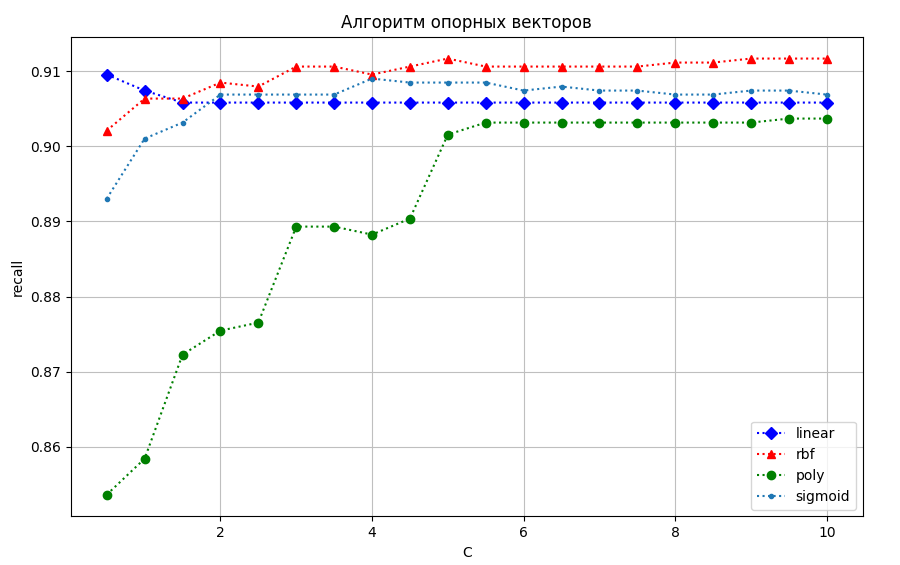
\includegraphics[width=\textwidth]{inc/img/svm-graphs.png}
	\caption{Значения метрики recall при различных конфигурациях параметров алгоритма опорных векторов}
	\label{res:svm-graphs}
\end{figure}

На основании полученных результатов можно сделать вывод о том, что наилучшие результаты классификации достигаются при использовании следующих параметров: $C$ = 5, $kernel$ = 'rbf'. 


\section{Алгоритм k-ближайших соседей}
Согласно документации Scikit-Learn, конструктор класса KNeighborsClassifier, описывающий модель классификатора с использованием алгоритма $k$-ближайших соседей, принимает  параметр $n\_neighbors$, характеризующих модель. Данный параметр описывает количество "соседей"\space, на основании которого принимается решение о принадлежности объекта тому или иному классу.

В данном случае можно также применить метод GridSearchCV, чтобы определить оптимальное значение параметра $n\_neighbors$, при котором классификатор будет давать наилучший результат.

На рисунке \ref{res:kn-graphs} представлен график зависимости метрики recall(полнота) классификатора в зависимости от значения параметра $n\_neighbors$.

\begin{figure}[h!]
	\centering
	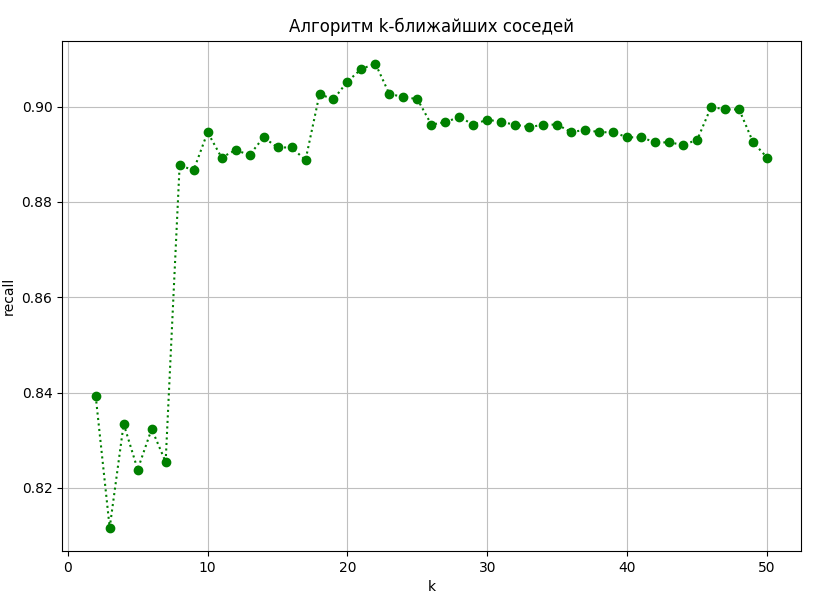
\includegraphics[width=\textwidth]{inc/img/kn-graphs.png}
	\caption{Значения метрики recall в зависимости от значения параметра $n\_neighbors$}
	\label{res:kn-graphs}
\end{figure}

На основании полученных результатов можно сделать вывод о том, что наилучшие результаты классификации достигаются при $n\_neighbors$ = 22.

\section{Сравнение алгоритмов классификации}

Ранее были проанализированы параметры алгоритмов $k$-ближайших соседей и опорных векторов, при которых классификатор выдает наилучший результат. Следует заметить, что при использовании алгоритма "наивной"\space байесовской классификации не используются какие-либо параметры, влияющие на работу классификации, соответственно нет необходимости отдельно исследовать работу данного алгоритма.

Ниже представлены результаты сравнения описанных алгоритмов классификации с использованием метрик: точность, полнота и f-мера. Все значения получены с использованием метода перекрестной проверки с разбиением исходной выборки на 5 частей. При обучении классификаторов использовались значения параметров, полученные в предыдущих разделах, за исключением "наивной"\space байесовской классификации, так как в данном случае такие параметры отсутствуют. 
Значения для точности (precision), полноты (recall) и f-меры представлены на рисунках \ref{res:precision}, \ref{res:recall}, \ref{res:f1} соответственно.

На основании полученных результатов, можно сделать вывод, что значения, полученные для алгоритмов опорных векторов и $k$-ближайших соседей, отличаются не значительно и данные являются наиболее подходящими для решения поставленной задачи по сравнению с алгоритмом "наивной"\space байесовской классификации.

\newpage
\begin{figure}[h!]
	\centering
	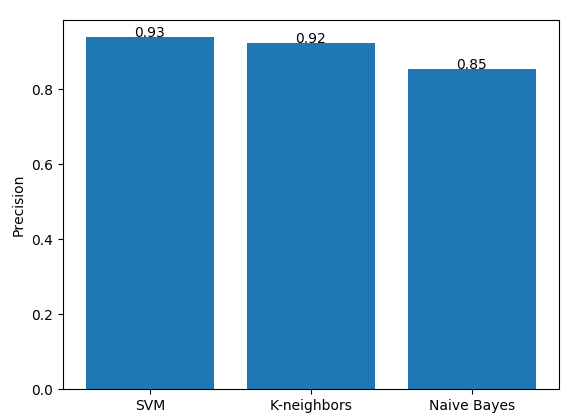
\includegraphics[scale=0.7]{inc/img/precision.png}
	\caption{Значения точности}
	\label{res:precision}
\end{figure}


\begin{figure}[h!]
	\centering
	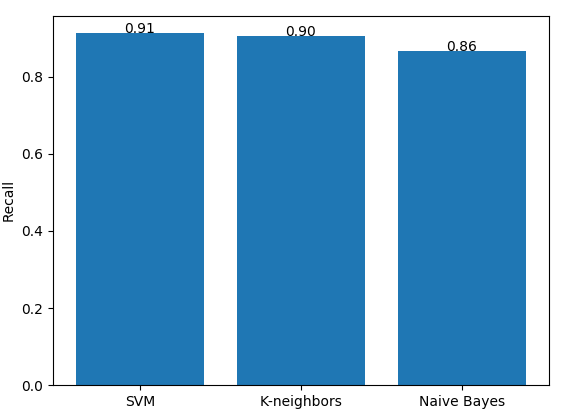
\includegraphics[scale=0.7]{inc/img/recall.png}
	\caption{Значения полноты}
	\label{res:recall}
\end{figure}

\newpage
\begin{figure}[h!]
	\centering
	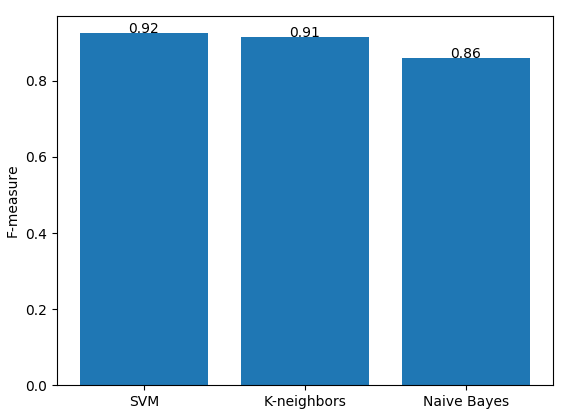
\includegraphics[scale=0.7]{inc/img/f1.png}
	\caption{Значения f-меры}
	\label{res:f1}
\end{figure}

\newpage
\section{Выводы}

В рамках проведенных исследований каждый из описанных алгоритмов классификации был проверен при различных конфигурациях параметров, предоставляемых используемой библиотекой, в целях выявления наилучшей конфигурации параметров модели.

Затем с использованием описанных ранее метрик было проведено сравнений алгоритмов классификации между собой. Полученные результаты свидетельствуют о том, что наиболее подходящими алгоритмами для решения данной задачи являются алгоритмы опорных векторов и $k$-ближайших соседей.


%%% Local Variables:
%%% mode: latex
%%% TeX-master: "rpz"
%%% End:
